%----------------------------------------
% Preamble to set up the document
%----------------------------------------
\documentclass{article}

% set up packages (you shouldn't need to touch this)
\usepackage{graphicx}  % required to insert images
\usepackage{hyperref}  % for hyperlinks
\usepackage[svgnames]{xcolor}  % to change hyperlink colors
\colorlet{linkcolour}{DarkBlue}
\hypersetup{colorlinks=true, linkcolor=linkcolour, citecolor=linkcolour, urlcolor=linkcolour,}

% additional packages:
\usepackage{amsmath}

% Margins
\topmargin=-0.45in
\evensidemargin=0in
\oddsidemargin=0in
\textwidth=6.5in
\textheight=9.0in
\headsep=0.25in

% use a sans serif font
\renewcommand{\familydefault}{\sfdefault}

%----------------------------------------
% Step 1: Edit the lecture title
%----------------------------------------
\title{
Lecture 3: Counting at Scale: MapReduce  \\  % Lecture title
Modeling Social Data, Spring 2017 \\   % Course title
Columbia University                    % School
}

%----------------------------------------
% Step 2: Edit your name and the date
%----------------------------------------
\author{Aarshay Jain}                     % Scribe's name
\date{February 3, 2017}                % Lecture date

\begin{document}

\maketitle


%----------------------------------------
% Step 3:
% Rename uni.tex to match your uni,
% edit the filename accordingly below,
% and put your notes in this file
%----------------------------------------
%----------------------------------------
% Lecture 3 notes
%----------------------------------------

\section*{Part1: Guest Lecture}

We would cover the following topics in today's class:
\begin{itemize}
    \item Computational Tractability: how to measure running time 
    \item Asymptotic order of growth: how to analyze and compare running times
    \item Common running times: typical data structures and algorithms
\end{itemize}

\section{Computational Tractability}
The running time is measured in terms of input size - n. The typical run times are:
\begin{itemize}
    \item $2^n$ (exponential)
    \begin{itemize}
        \item generally brute force algorithms have exponential running times
        \item this running time is not ideal as problems become practically unsolvable for even small running times
    \end{itemize}
    \item $cn^d,\ c,d>0$ (polynomial)
    \begin{itemize}
        \item polynomial time algorithms are considered to be theoretical efficient and theoreticians stop here
        \item but practically, the constants c,d matter. for example, if we compare $20n^100$ and $n^{1+0.02log(n)}$, the later is prefered though is exponential because the former polynomial runtime has very high coefficients.
    \end{itemize}
    \item Order of growth: $ n < n log(n) < n^2 < n^3 < 1.5^n < 2^n < n! $
    \begin{itemize}
        \item there are some sub-linear algorithms as well which are better than linear but are mostly approximate algorithms
        \item the ideal range for an algo is below $n^2$ as anything beyond that becomes difficult to handle as data size increases
    \end{itemize}
\end{itemize}

Different types of analysis of run-time can be performed as following:
\begin{itemize}
    \item Worst Case Analysis: this is most commonly used and compares algorithms on asymptotic performance
    \item Average Case Analysis: here we analyze how the algo performs on average. we need some sense of the number of times a particular operation is expected to be run to be able to get the average
    \item Amortized Analysis: here the time taken by a sequence of operations is analyzed
    \item These 3 can be compared using the example of push and popall into a stack. A stack is a LIFO (last in first out) data structure.
    \begin{itemize}
        \item Worst case: push - $O(1)$ | popall - $O(n)$
        \item Average Case: if popall is a rarely called, then average runtime is $O(1)$
        \item Amortized: a popall operation will take only as much time as the number of push operations before it. So a sequence of push and popall will take $O(1)$ amortized time. This can be understood as every push operation investing 1\$ in the bank on each call and popall using that invested money to perform the operation. So the amortized cost is constant.
    \end{itemize}
\end{itemize}

\section{Asymptotic Order of Growth}

Three types of notations can be used for asymptotic analysis. These are:
\subsection{Big-Oh ($O$) - Upper Bounds}
This specifies the upper bound on the running time of an algorithm. The runtime T(n) can be written as:
$$ T(n)\ =\ O(f(n))\ if \exists\ c>0, n_0 \ge 0 $$
$$ s.t.\ T(n) \le c.f(n),\ \forall\ n>n_0 $$

Example: $T(n)=32n^2+17n+1\ ==>\ T(n)=O(n^2)$ This can be verified by taking any c greater than 32 say c=50 and $n_0$=1

Note that theoretically $T(n)\subset O(f(n))$ but using $T(n) = O(f(n))$ is accepted in the computer science community.

\subsection{Big-Omega ($\Omega$) - Lower Bounds}
This specifies the lower bound on the running time of an algorithm. The runtime T(n) can be written as:
$$ T(n)\ =\ \Omega(f(n))\ if \exists\ c>0, n_0 \ge 0 $$
$$ s.t.\ T(n) \ge c.f(n),\ \forall\ n>n_0 $$

Example: $T(n)=32n^2+17n+1\ ==>\ T(n)=\Omega(n)=\Omega(n^2)$

\subsection{Big-Theta ($\Theta$) - Tight Bounds}
This specifies a tight bound on the running time of an algorithm, i.e. an order of polynomial which can be both an upper and lower bound with different constants. The runtime T(n) can be written as:
$$ T(n)\ =\ \Theta(f(n))\ if \exists\ c_1,c_2>0, n_0 \ge 0 $$
$$ s.t.\ c_1.f(n) \le T(n) \le c_2.f(n),\ \forall\ n>n_0 $$

Example: $T(n)=32n^2+17n+1\ ==>\ T(n)=\Theta(n^2)$ as $n^2$ is both an upper as well as a lower bound

\subsection{Rules of Thumb}
The following rules can be typically applied when determining the running time:
\begin{enumerate}
    \item $T(n)=a_0+a_1n+a_2n^2+...+a_dn^d\ ==>\ T(n)=\Theta(n^d)$
    \item $O(log_a n) = O(log_b n),\ a,b>0 $ [base of log doesn't matter because base change involes a constant factor]
    \item $ n^d=O(r^n),\ \forall\ r>1,d>0$ [any polynomial runtime will be dominated by exponential asymptotically]
\end{enumerate}

\section{Common Running Times}
Now lets understand some common running times.

\subsection{$O(n)$ - linear}
The algo iterates over all the entries of the data a constant number of times. Eg: max, sum, min, etc.

Note: This assumes that constant time is spent at every iteration. But note that any number K requires $log_2(K)$ bits to be represented so it takes $log_2(K)$ time at each index. However, modern computers perform all these tasks in parallel so we can ignore this effect.

\subsection{$O(nlogn)$}
This is generally the runtime of divide and conquer algorithms like sorting. Figure \ref{fig:divide_n_conquer} illustrates the concept well.

\begin{figure}[ht]
  \begin{center}
    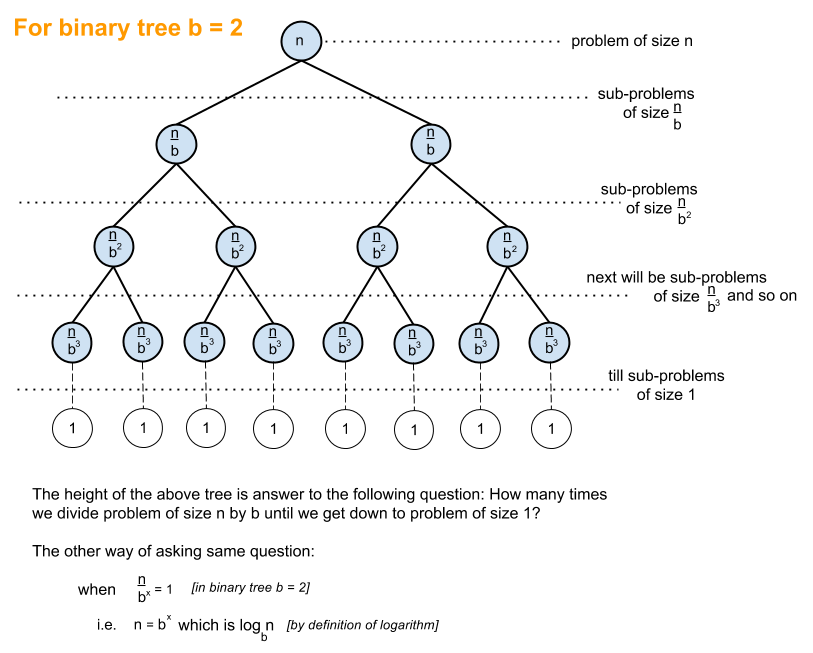
\includegraphics[width=0.5\textwidth]{figures/divide_n_conquer.png}
    \caption{Working of divide and conquer algorithms \protect\footnotemark when problem gets divided into 2 sub-problems at each step}
    \label{fig:divide_n_conquer}
  \end{center}
\end{figure}
\footnotetext{\url{https://i.stack.imgur.com/spHFh.png}}

Key observations:
\begin{itemize}
    \item each problem gets divided into 2 sub-problems at each step
    \item at any particular step (horizontal layer), equal amount, i.e. $O(n)$ time is being spent
    \item there are $O(log_2(n))$ such layers
    \item so total time is $O(nlogn)$ [note: base of log doesn't matter in big-oh notations]
\end{itemize}

Note: it has been proven that any comparison-based sorting algorithm can't do better than $O(nlogn)$.

\subsection{$O(n^2)$ - quadratic}
In this case, all of the n observations are iterated over a some linear function of n. So total time is quadratic. Eg: bubble sort, quick sort

\subsection{$O(n^3)$ - cubic}
Example: counting the number of triangles in graphs or number of triplets in a node.

Note: matrix multiplication of two nxn matrices is cubic in n but the input is not really n but $n^2$. So its debatable whether these are cubic runtime algorithms or not.

\subsection{$O(logn)$}
These are highly efficient algorithms which run without even scanning the full array once. Example: binary search on sorted arrays, binary tree search on balanced trees

\subsection{Hash Tables}
They allow searching in near constant time. Figure \ref{fig:hash_table} describes the working of hash tables.

\begin{figure}[ht]
  \begin{center}
    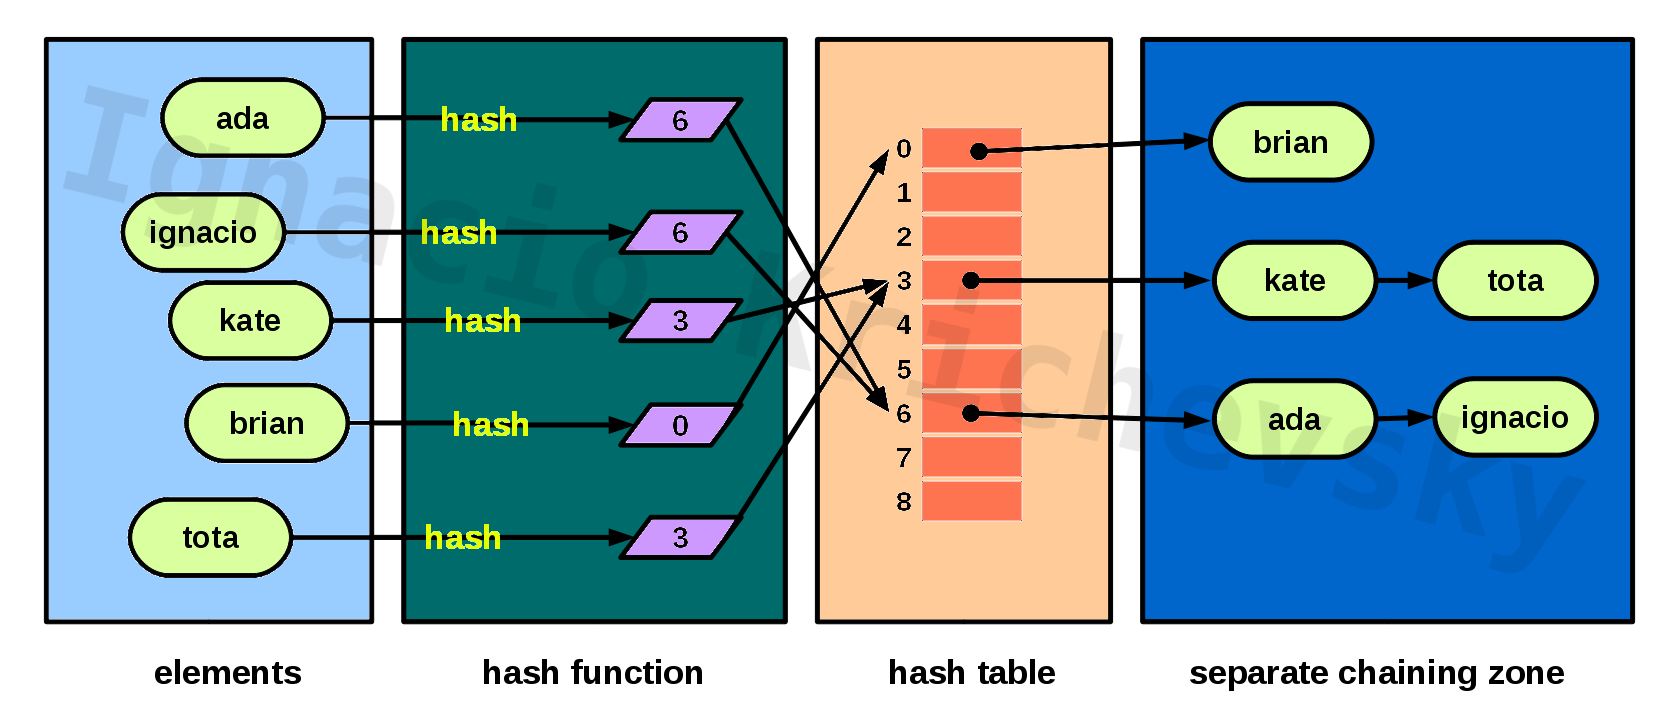
\includegraphics[width=0.5\textwidth]{figures/hash_table.png}
    \caption{Working of hash tables with chaining \protect\footnotemark}
    \label{fig:hash_table}
  \end{center}
\end{figure}
\footnotetext{\url{http://krichevsky.com.ar/root/programming/data\%20structures\%20&\%20algorithms/hashTableWithSeparateChaining.png}}

It works as following:
\begin{itemize}
    \item a hash function h converts an input element into an index of the hash table where it is stored
    \item the function h randomizes the placement of items so that each element has equal probability of being at any index in the hash table
\end{itemize}

An idea hash function is the one which gives a unique index to each element. If all the elements are known beforehand, then its possible to define such a hash function. But if the inputs are unknown, then there might be collisions in the hash table, i.e. multiple elements being hashed to the same index.

A collision occurs when $\exists k1,k2\ s.t.\ h(k1)=h(k2)\ but\ k1 \ne k2$. When this happens, a chain is formed at the index of collision as shown in Figure \ref{fig:hash_table}. The expected number of collisions depend on the number of items (n) to be hashed and the size of the hash table (t). 

\begin{align*}
    p(collision) &= \frac{1}{n} \\
    E(\#collisions) &= \binom{n}{2} \frac{1}{n} = O(n)
\end{align*}

Thus, the expected number of collisions per bin is $O(1)$. Typically, the size of the hash table is kept slightly bigger than n.

\subsection{Joining tables}

Problem: Given 2 tables A and B with a common columns say ID, we need to merge the rows with same IDs together. There are various ways to solve the problem:

\begin{itemize}
    \item For every ID in table A, search in entire table B for matching ID and merge. This takes $O(n^2)$ time
    \item Create an index on the ID column for table B. Now for every element in table A, we can search for an element in table B in $O(logn)$ time. So the total time is $O(nlogn)$.
    \item Create a hash function which maps IDs into a hash table. Push IDs of table A into the hash table. Then for every ID in table B, push it to the hash table and combine the data with that of table A in the same index. This gives a $O(n)$ time algorithm for joining.
    \item If both the ID columns of table A and table B can be sorted, then you can simply walk through the IDs in linear time and merge.
\end{itemize}

\section*{Part2 - Data Manipulation in R using tidyverse}

In this section, I'll try to augment the content of slides with additional information discussed in class. The notes are referenced by slide number of the updated slides on GitHub repository:

\begin{itemize}
    \item Slide \#5:
    \begin{itemize}
        \item factor variables are coded as numeric in the background and appears as labels to the user. we can do str(variable\_name) to know the real structure.
    \end{itemize}
    
    \item Slide \#6:
    \begin{itemize}
        \item dataframes are different from matrices in the same way as lists are from vectors. matrices accept data of single type but different columns of dataframes can have different types of data.
    \end{itemize}
    
    \item Slide \#10:
    \begin{itemize}
        \item In this slide, N: \#rows, K: \#columns
        \item for-loops are constructs in R but we should try to avoid them as much as possibe. These functions give faster ways of acheiving the same objective as for-loops. If you're using a for-loop, you're probably missing a trick.
        \item All functions, except group\_by, are not inplace, i.e. they won't affect the original dataframe but return a new dataframe which can be stored different or overwritten on the old dataframe.
    \end{itemize}
    
    \item Slide \#11:
    \begin{itemize}
        \item Note that here "start\_station\_name" is not a variable in the R environment but the name of a column. 
        \item filter would first try to parse this as a column in the dataframe trips and if not found then it will look into the global environment. So you've to be careful if you have variable names which are same as column names.
        \item the same concept applies to other functinos as well.
    \end{itemize}
    
\end{itemize}

Finally, some notes on the "wierdness" of R over general programming languages:

\begin{itemize}
    \item it uses "$<-$" as an assignment operator and not "=". Even "=" works but there is some difference in the background.
    \item there are some datasets which are lurking in the background but you don't see them in your environment unless you explicitly save them in a variable. For example "head(iris)" will give you the top 6 rows of the iris dataset which might not even by in your environment. "iris $<-$ iris" will save it in your environment as well.
    \item "\$" can be used to index columns but try to avoid it
    \item comparison operators "\&" and "\&\&" are different. Former works vectorized, i.e. element by element while later works considering every operand as a single element.
    \item \%$>$\% are R's version of pipes we saw in unix
\end{itemize} 

\end{document}

%%% Local Variables:
%%% mode: latex
%%% TeX-master: t
%%% End:
